\documentclass[a4paper]{article}
\usepackage[utf8]{inputenc}
\usepackage[spanish, es-tabla, es-noshorthands]{babel}
\usepackage[table,xcdraw]{xcolor}
\usepackage[a4paper, footnotesep = 1cm, width=20cm, top=2.5cm, height=25cm, textwidth=18cm, textheight=25cm]{geometry}
%\geometry{showframe}

\usepackage{tikz}
\usepackage{amsmath}
\usepackage{amsfonts}
\usepackage{amssymb}
\usepackage{float}
\usepackage{graphicx}
\usepackage{caption}
\usepackage{subcaption}
\usepackage{multicol}
\usepackage{multirow}
\setlength{\doublerulesep}{\arrayrulewidth}
\usepackage{booktabs}
\usepackage{mathrsfs,amsmath}
\usepackage{hyperref}
\hypersetup{
    colorlinks=true,
    linkcolor=blue,
    filecolor=magenta,      
    urlcolor=blue,
    citecolor=blue,    
}

\newcommand{\quotes}[1]{``#1''}
\usepackage{array}
\newcolumntype{C}[1]{>{\centering\let\newline\\\arraybackslash\hspace{0pt}}m{#1}}
\usepackage[american]{circuitikz}
\usetikzlibrary{calc}
\usepackage{fancyhdr}
\usepackage{units} 

\graphicspath{./Imagenes}

\pagestyle{fancy}
\fancyhf{}
\lhead{22.05 ASSD}
\rhead{Mechoulam, Lambertucci, Rodriguez, Londero}
\rfoot{Página \thepage}

\begin{document}
En este punto se analizará la utilización del remuestreo en una señal de AM descrita por la siguiente ecuación:
\begin{equation}
X_c = A_{MAX} \cdot \left[ \frac{1}{2} \cdot \cos (2 \pi (1.8 f_{in}) t) +\cos (2 \pi (2 f_{in}) t)  + \frac{1}{2} \cdot \cos (2 \pi (2.2 f_{in}) t) \right]
\end{equation}
Lo que se busca con el remuestreo es emular un muestreo ideal, esto se lleva a cabo al utilizar en conjunto el Sample and Hold y la llave analógica, de tal manera que la llave se encuentre cerrada mientras que  se encuentra en Hold y abierta durante el Sample. Resulta simple notar, que es equivalente a multiplicar la señal por un tren de deltas y luego convolucionar la señal con un pulso.
	
\begin{figure}[H]
	\centering
	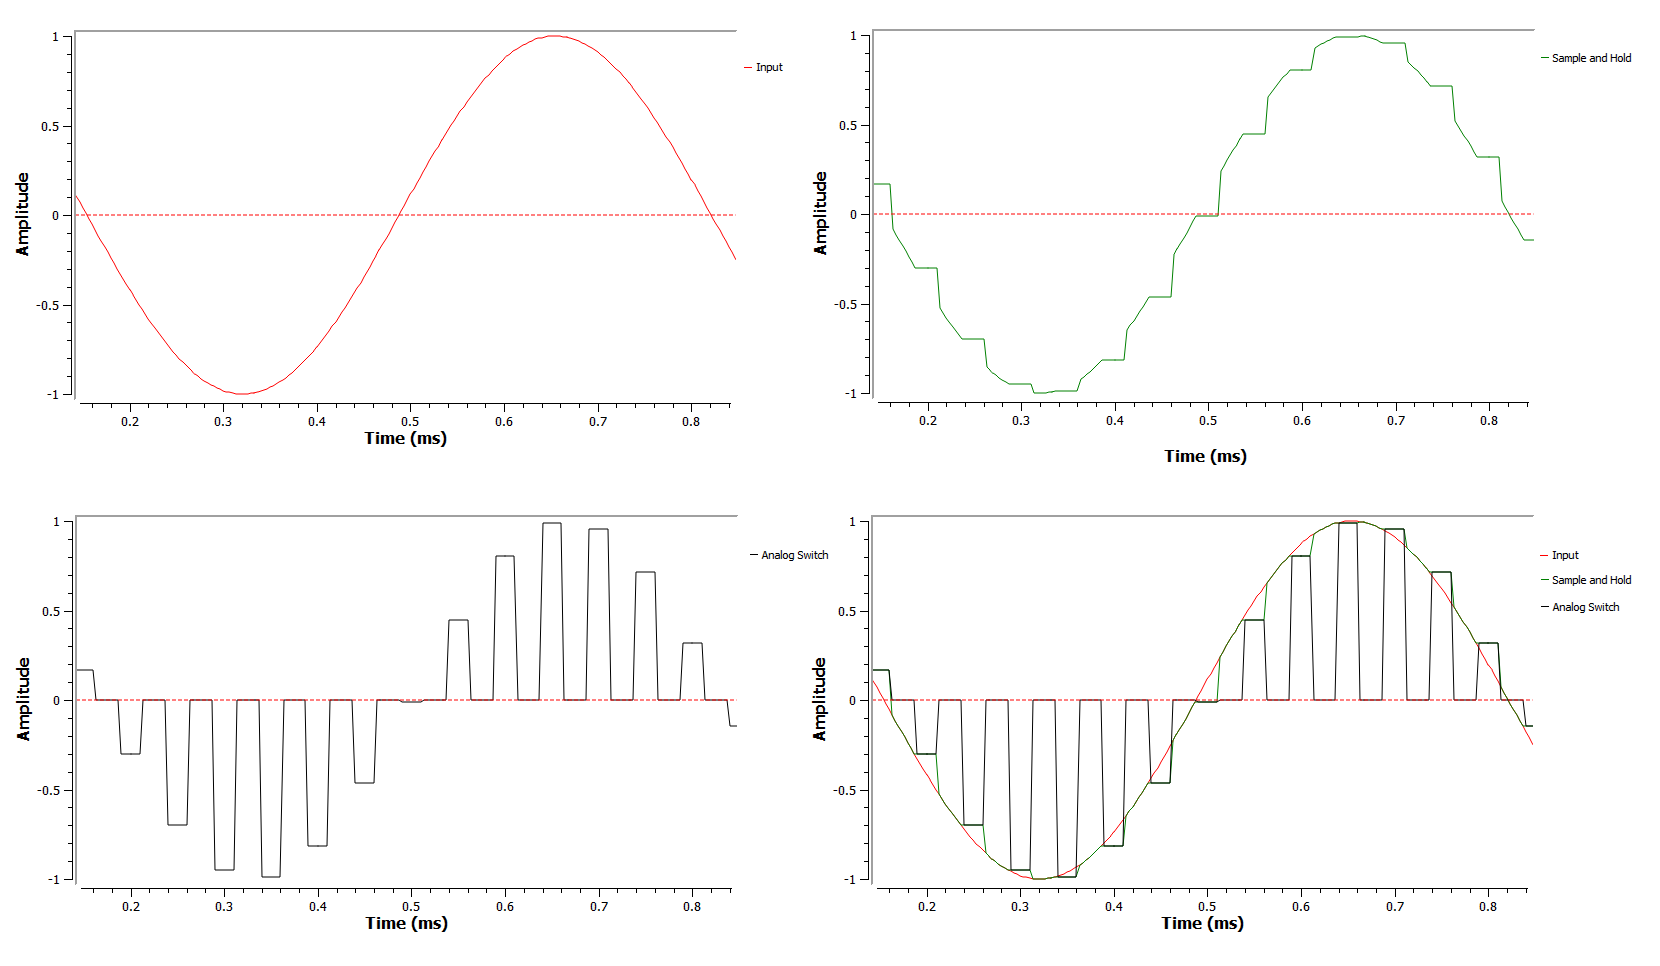
\includegraphics[width=1\textwidth]{ImagenesEjercicio7/t1.PNG}
\caption{Señal senoidal en sus diversas etapas de muestreo.}
	\label{fig:muestreo}
\end{figure}
Luego consideraremos que las señales, dado que $f_{in} = 1.5kHz$ , tendrán una frecuencia $f_p=3kHz$ y $f_m=300Hz$ con un m=1, esto define que la máxima frecuencia del sistema será de 3.3kHz, por Nyquist la frecuencia de muestreo debe ser por lo menos de 6.6kHz, se decidió utilizar una $f_s = 15kHz$. lo cual implica un período de 34$\mu$s, es de interés saber que el tiempo de adquisición  del SH es típicamente de \href{http://www.ti.com/lit/ds/symlink/lf398-n-mil.pdf}{6$\mu$s}, por seguridad se dejara un margen de error para el sample, dejando para este el $12\mu s$, a partir de aquí se puede determinar que debe estar en Sample un 35$\%$ y por lo tanto la llave analógica debe tener un Duty cycle del 65$\%$, siendo conscientes de que a mayor Duty cycle mayor será la potencia recuperada de la señal.
\\
Finalmente se grafica la tensión en cada uno de los nodos del sistema dada la entrada AM $X_c$.
\begin{figure}[H]
	\centering
	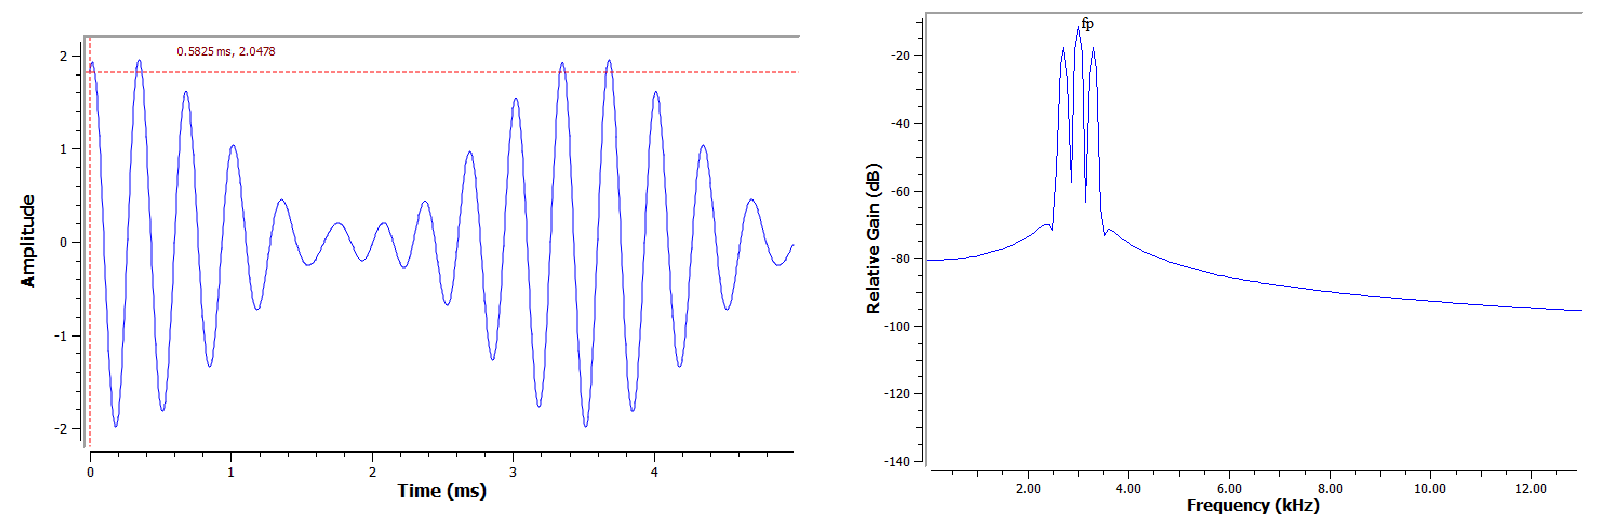
\includegraphics[width=1\textwidth]{ImagenesEjercicio7/input.PNG}
\caption{Señal de entrada AM.}
	\label{fig:input}
\end{figure}
\begin{figure}[H]
	\centering
	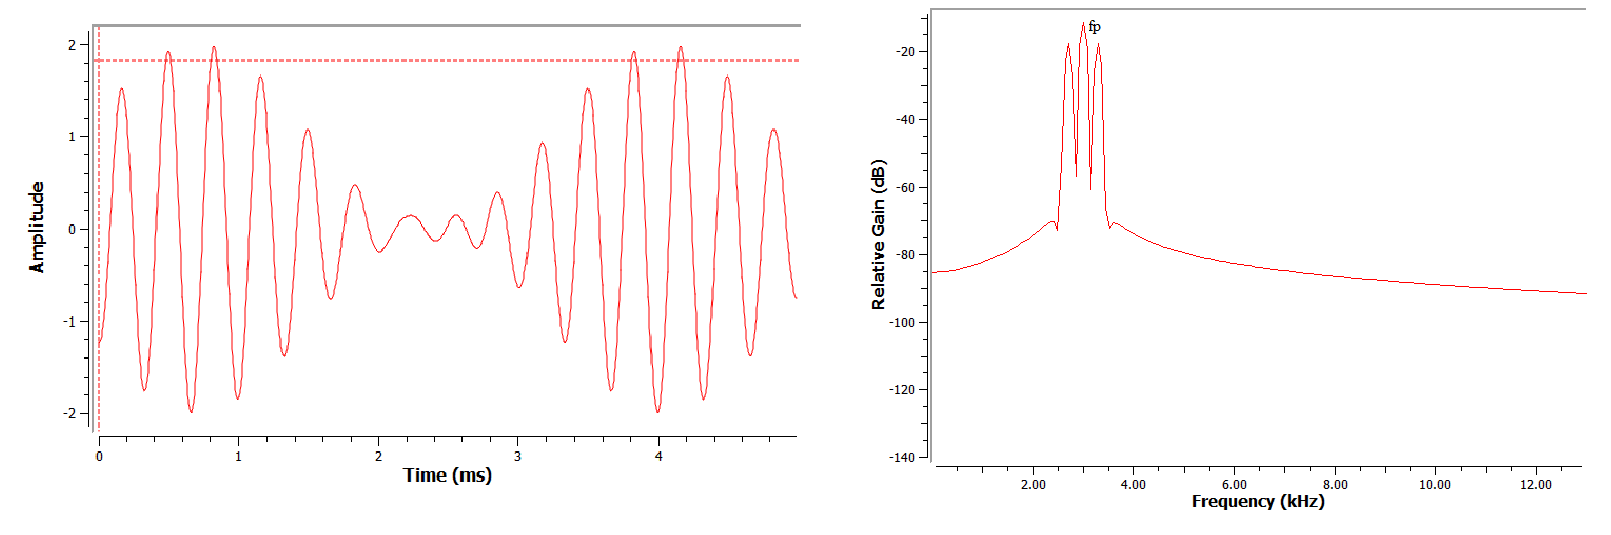
\includegraphics[width=1\textwidth]{ImagenesEjercicio7/alias.PNG}
\caption{Señal luego del filtro anti alias.}
	\label{fig:alias}
\end{figure}
\begin{figure}[H]
	\centering
	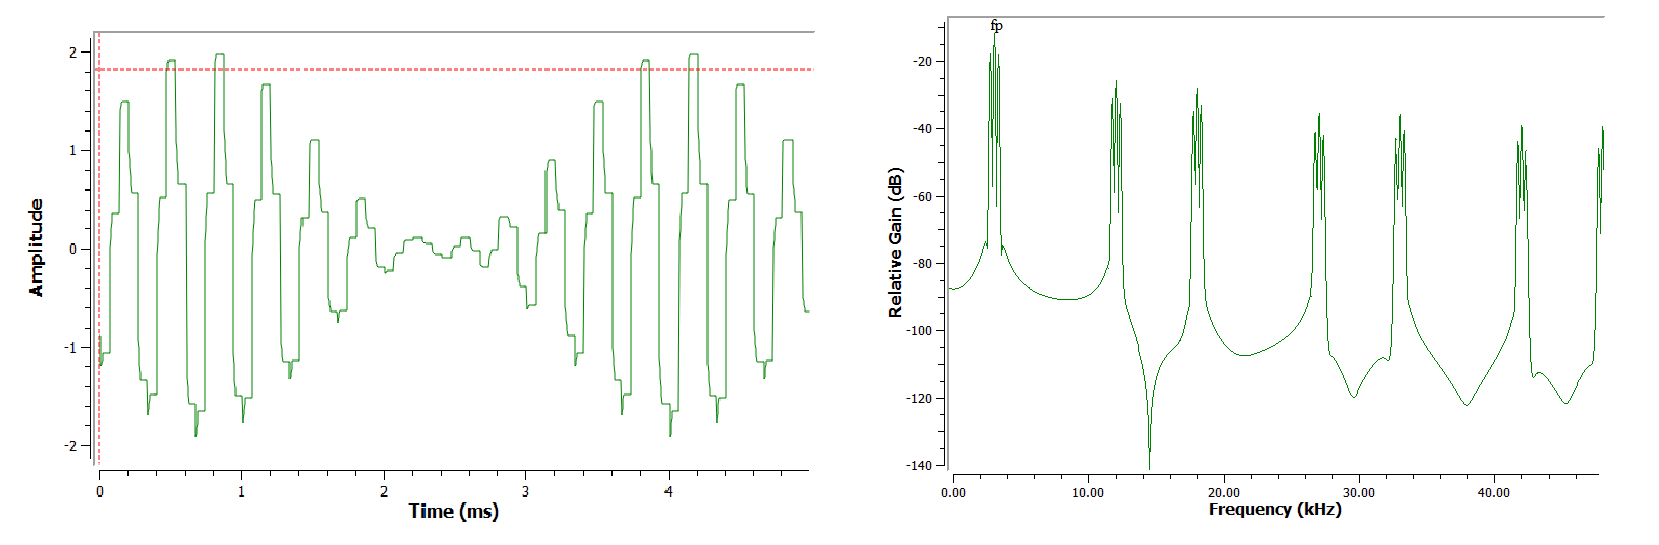
\includegraphics[width=1\textwidth]{ImagenesEjercicio7/sh.PNG}
\caption{Señal luego del Sample and Hold.}
	\label{fig:sh}
\end{figure}
\begin{figure}[H]
	\centering
	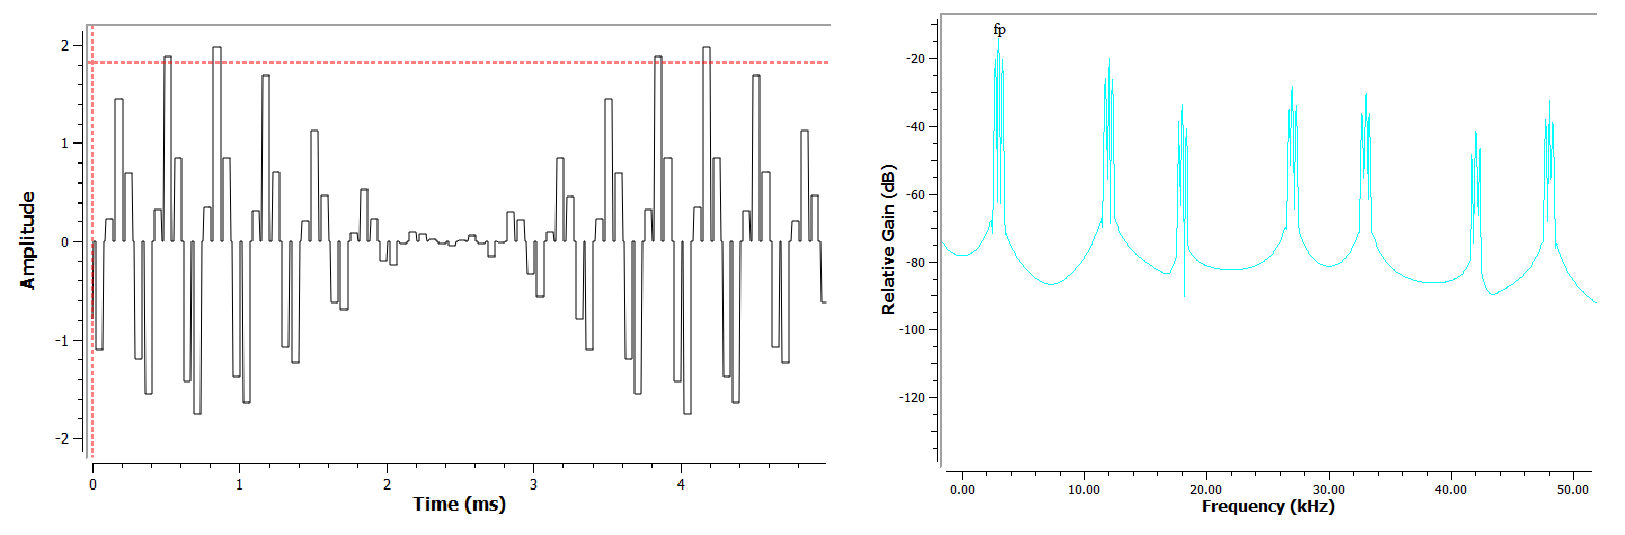
\includegraphics[width=1\textwidth]{ImagenesEjercicio7/analog.PNG}
\caption{Señal luego de la llave analógica.}
	\label{fig:analog}
\end{figure}
\begin{figure}[H]
	\centering
	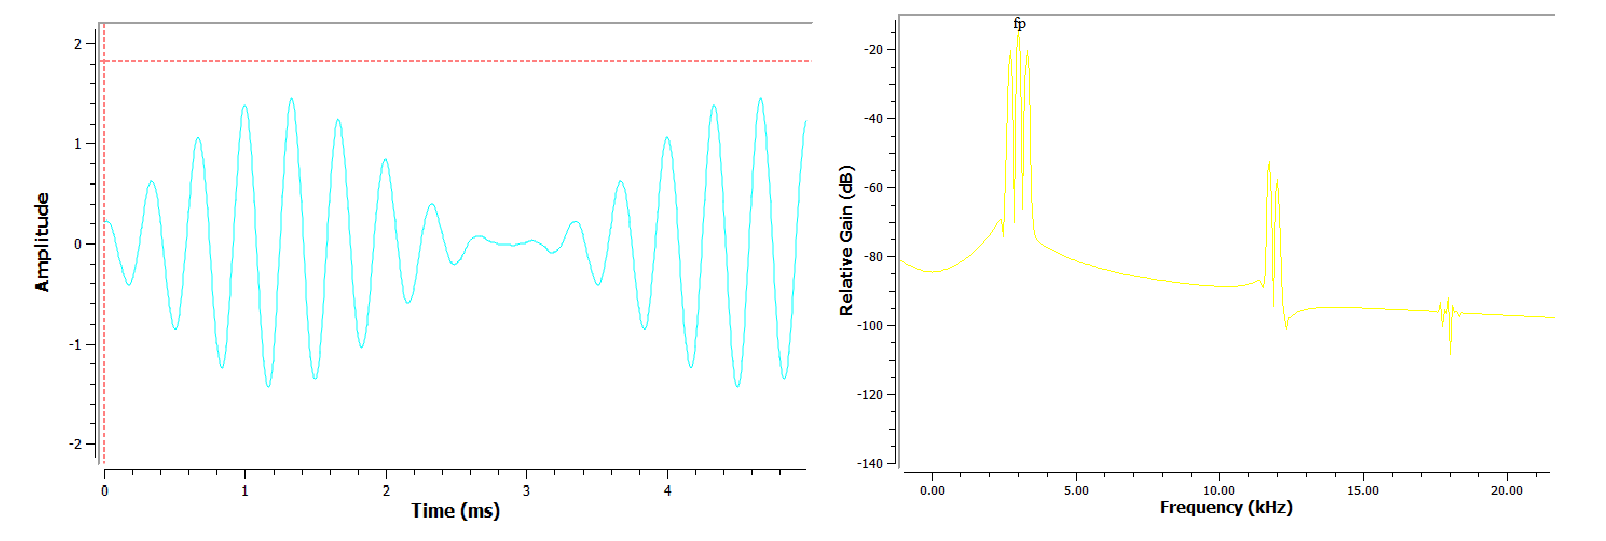
\includegraphics[width=1\textwidth]{ImagenesEjercicio7/recovery.PNG}
\caption{Señal luego del filtro recuperador.}
	\label{fig:recovery}
\end{figure}
Es apreciable, que el espectro de cada señal correpsonde con el de una señal modulada en AM para las figuras (\ref{fig:input}) , (\ref{fig:alias}) y (\ref{fig:recovery}) mientras que se ve en las figuras (\ref{fig:sh}) y (\ref{fig:analog}) las replicas del espectro original en el resto del espectro.
\end{document}